\documentclass[12pt,a4paper]{article}
\usepackage[utf8]{inputenc}
\usepackage{amsmath, amssymb}
\usepackage{graphicx}
\usepackage{geometry}
\usepackage{float}
\usepackage{booktabs}
\usepackage{circuitikz}
\usepackage{caption}
\geometry{a4paper, margin=1in}

\title{\textbf{11. Schmitt Trigger using OP-Amp}}
\author{Yamulapalli Nandu Navadeep \\ Roll Number: IMS24267}
\date{Date of Experiment: 19/08/2026 \\ Date of Submission: \today}

\begin{document}

\maketitle

\section{Aim of the Experiment}
To design a Schmitt trigger using IC 741 for a specified Lower Threshold Point (LTP) and Upper Threshold Point (UTP) and to plot the hysteresis curve.

\section{Theory}
A Schmitt trigger is a comparator circuit with hysteresis. It is often called a squaring circuit because it converts an irregular shaped input waveform into a square wave. The output voltage changes its state every time the input voltage crosses certain threshold levels.

The input voltage at which the output switches from positive saturation ($+V_{sat}$) to negative saturation ($-V_{sat}$) is called the Upper Triggering Point or Upper Threshold Point (UTP). Similarly, the input voltage at which the output switches back from $-V_{sat}$ to $+V_{sat}$ is called the Lower Triggering Point or Lower Threshold Point (LTP).

These threshold voltages are determined by the voltage divider network formed by resistors $R_1$ and $R_2$. When the output is at $+V_{sat}$, the voltage across $R_1$ gives the UTP:
$$ V_{UTP} = \frac{R_1}{R_1 + R_2} (+V_{sat}) $$
When the input voltage exceeds $V_{UTP}$, the output switches to $-V_{sat}$. At this state, the voltage across $R_1$ gives the LTP:
$$ V_{LTP} = \frac{R_1}{R_1 + R_2} (-V_{sat}) $$
When the input voltage drops below $V_{LTP}$, the output switches back to $+V_{sat}$. The difference between the upper and lower threshold points creates a hysteresis loop.

\section{Procedure}
\begin{enumerate}
    \item Verify whether the op-amp IC is in good working condition by using it as a voltage follower.
    \item Set up the circuit on the breadboard as per the circuit diagram.
    \item Apply a sinusoidal input signal ($1\text{ kHz}$, $15\text{ V}$ peak) from the function generator.
    \item Connect the input to one channel and the output to the other channel of the CRO. Observe both waveforms simultaneously.
    \item Design the circuit for different values of LTP and UTP by changing the values of resistors $R_1$ and $R_2$.
    \item Measure the upper and lower threshold voltages from the CRO screen for each combination of resistors.
    \item Observe the transfer characteristics by switching the CRO to XY mode and plot the hysteresis curve.
\end{enumerate}

\section{Circuit Diagram}
\begin{figure}[H]
\centering
\begin{circuitikz}[scale=1, transform shape]
    % Op-Amp
    \draw (0,0) node[op amp] (OA) {IC 741};
    
    % Power supplies
    \draw (OA.up) -- ++(0,0.5) node[above] {$+15\text{ V}$ (7)};
    \draw (OA.down) -- ++(0,-0.5) node[below] {$-15\text{ V}$ (4)};
    
    % Input Vin to inverting terminal (-)
    \draw (OA.-) to[R, l=$R_1 || R_2$] ++(-3,0) coordinate (Vin_node);
    \draw (Vin_node) to[sV, l=$V_{in}$] ++(0,-2) node[ground]{};
    
    % Non-inverting terminal (+) routing R1 to ground leftwards
    \draw (OA.+) to[short, *-] ++(-1,0) to[R, l=$R_1$] ++(0,-2) node[ground]{};
    
    % Feedback R2 from Vout to (+) routing downwards
    \draw (OA.+) -- ++(0,-1.5) coordinate (fb) to[R, l_=$R_2$] (fb -| OA.out) -- (OA.out);
    
    % Output
    \draw (OA.out) to[short, *-o] ++(1,0) node[right] {$V_{out}$};
    
\end{circuitikz}
\caption{Circuit diagram of Schmitt Trigger using IC 741}
\end{figure}

\section{Waveforms and Transfer Characteristics}
\begin{figure}[H]
\centering
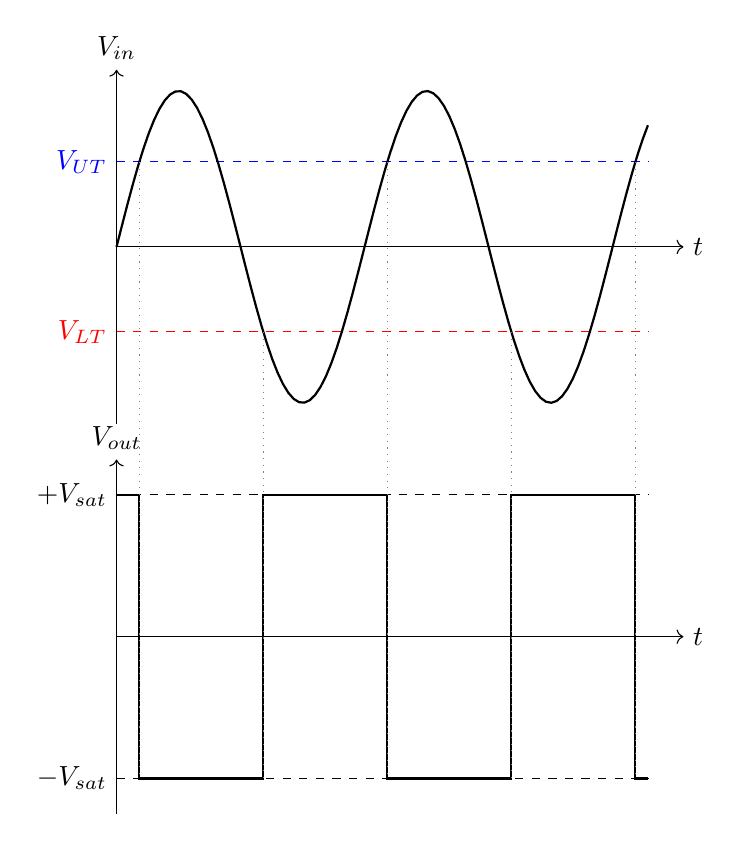
\begin{tikzpicture}[scale=0.9]
    % Axes for Vin
    \draw[->] (0,0) -- (8,0) node[right] {$t$};
    \draw[->] (0,-2.5) -- (0,2.5) node[above] {$V_{in}$};
    
    % VUT and VLT lines
    \draw[dashed, blue] (0,1.2) node[left] {$V_{UT}$} -- (7.5,1.2);
    \draw[dashed, red] (0,-1.2) node[left] {$V_{LT}$} -- (7.5,-1.2);
    
    % Sine wave for Vin
    \draw[thick, domain=0:7.5, samples=100] plot (\x, {2.2*sin(\x*360/3.5)});
    
    % Axes for Vout (shifted down)
    \begin{scope}[yshift=-5.5cm]
        \draw[->] (0,0) -- (8,0) node[right] {$t$};
        \draw[->] (0,-2.5) -- (0,2.5) node[above] {$V_{out}$};
        
        \draw[dashed] (0,2) node[left] {$+V_{sat}$} -- (7.5,2);
        \draw[dashed] (0,-2) node[left] {$-V_{sat}$} -- (7.5,-2);
        
        % Square wave for Vout
        \draw[thick] (0, 2) -- (0.32, 2) -- (0.32, -2) -- (2.07, -2) -- (2.07, 2) -- (3.82, 2) -- (3.82, -2) -- (5.57, -2) -- (5.57, 2) -- (7.32, 2) -- (7.32, -2) -- (7.5, -2);
    \end{scope}
    
    % Guidelines
    \draw[dotted, gray] (0.32, 1.2) -- (0.32, -7.5);
    \draw[dotted, gray] (2.07, -1.2) -- (2.07, -7.5);
    \draw[dotted, gray] (3.82, 1.2) -- (3.82, -7.5);
    \draw[dotted, gray] (5.57, -1.2) -- (5.57, -7.5);
    \draw[dotted, gray] (7.32, 1.2) -- (7.32, -7.5);

\end{tikzpicture}
\caption{Input and Output waveforms of the Schmitt Trigger}
\end{figure}

\begin{figure}[H]
\centering
\begin{tikzpicture}[scale=1.5]
    % Axes
    \draw[->] (-3,0) -- (3,0) node[right] {$V_{in}$};
    \draw[->] (0,-2.5) -- (0,2.5) node[above] {$V_{out}$};
    
    % VUT and VLT markers
    \draw (1.5, 0.1) -- (1.5, -0.1) node[below] {$V_{UT}$};
    \draw (-1.5, 0.1) -- (-1.5, -0.1) node[below] {$V_{LT}$};
    
    % +Vsat and -Vsat markers
    \draw (0.1, 1.8) -- (-0.1, 1.8) node[below right] {$+V_{sat}$};
    \draw (0.1, -1.8) -- (-0.1, -1.8) node[above right] {$-V_{sat}$};
    
    % Hysteresis loop - Increasing Vin (Bottom path then jump up)
    % Sticking out bottom-left
    \draw[thick, blue, ->] (-2.5, -1.8) -- (-1.5, -1.8);
    % Inside loop bottom
    \draw[thick, blue, ->] (-1.5, -1.8) -- (0, -1.8);
    \draw[thick, blue] (0, -1.8) -- (1.5, -1.8);
    % Right vertical jump
    \draw[thick, blue, ->] (1.5, -1.8) -- (1.5, 0);
    \draw[thick, blue] (1.5, 0) -- (1.5, 1.8);
    % Top right outgoing 
    \draw[thick, blue] (1.5, 1.8) -- (2.5, 1.8);
    
    % Hysteresis loop - Decreasing Vin (Top path then drop down)
    % Sticking out top-right
    \draw[thick, red, ->] (2.5, 1.8) -- (1.5, 1.8);
    % Inside loop top
    \draw[thick, red, ->] (1.5, 1.8) -- (0, 1.8);
    \draw[thick, red] (0, 1.8) -- (-1.5, 1.8);
    % Left vertical drop
    \draw[thick, red, ->] (-1.5, 1.8) -- (-1.5, 0);
    \draw[thick, red] (-1.5, 0) -- (-1.5, -1.8);
    % Bottom left outgoing 
    \draw[thick, red] (-1.5, -1.8) -- (-2.5, -1.8);
    
    % Add text to explain arrows
    \node[blue, right] at (1.5, 0.9) {Input increasing};
    \node[red, left] at (-1.5, -0.9) {Input decreasing};

\end{tikzpicture}
\caption{Transfer characteristics (Hysteresis curve) of the Schmitt Trigger}
\end{figure}

\section{Tabular Column}
\begin{table}[H]
\centering
\begin{tabular}{|c|c|c|c|c|c|c|c|}
\hline
\textbf{$R_1$} & \textbf{$R_2$} & \multicolumn{2}{c|}{\textbf{Designed (V)}} & \multicolumn{2}{c|}{\textbf{Measured (V)}} & \textbf{$H_{Theo}$ (V)} & \textbf{$H_{meas}$ (V)} \\
\cline{3-6}
& & \textbf{UTP} & \textbf{LTP} & \textbf{UTP} & \textbf{LTP} & & \\
\hline
$5.4\text{ k}\Omega$ & $10\text{ k}\Omega$ & $5.5$ & $-5.5$ & $5.6$ & $-5.6$ & $5.5$ & $5.75$ \\
$1.5\text{ k}\Omega$ & $10\text{ k}\Omega$ & $2.0$ & $-2.0$ & $2.9$ & $-2.3$ & $2.0$ & $2.15$ \\
$10\text{ k}\Omega$ & $47\text{ k}\Omega$ & $2.7$ & $-2.7$ & $3.5$ & $-3.1$ & $2.7$ & $3.8$ \\
$10\text{ k}\Omega$ & $56\text{ k}\Omega$ & $2.3$ & $-2.3$ & $3.2$ & $-2.7$ & $2.3$ & $3.4$ \\
$1.5\text{ k}\Omega$ & $5.4\text{ k}\Omega$ & $3.33$ & $-3.33$ & $4.0$ & $-3.4$ & $3.33$ & $4.0$ \\
\hline
\end{tabular}
\caption{Observations for Schmitt Trigger Thresholds}
\end{table}

\section{Calculations}
The theoretical threshold voltages are calculated using the formula:
$$ V_{UT} = \frac{R_1}{R_1 + R_2} (+V_{sat}) $$
$$ V_{LT} = \frac{R_1}{R_1 + R_2} (-V_{sat}) $$
Assuming the practical saturation voltage of the op-amp is approximately $\pm 15.7\text{ V}$ (which corresponds to the expected values):

For $R_1 = 5.4\text{ k}\Omega$ and $R_2 = 10\text{ k}\Omega$:
$$ V_{UT} = \frac{5.4}{5.4 + 10} \times 15.7 \approx 5.5\text{ V} $$
$$ V_{LT} = \frac{5.4}{5.4 + 10} \times (-15.7) \approx -5.5\text{ V} $$

\section{Results}
The Schmitt trigger circuit was successfully designed and set up using the IC 741 operational amplifier. The Upper Threshold Point (UTP) and Lower Threshold Point (LTP) were measured for various combinations of resistors $R_1$ and $R_2$. The measured threshold values were found to be close to the theoretical design values. The hysteresis curve was also successfully observed on the CRO in XY mode.

\section{Error Calculation}
Taking the first set of readings ($R_1 = 5.4\text{ k}\Omega$, $R_2 = 10\text{ k}\Omega$):
Theoretical $V_{UT} = 5.5\text{ V}$
Measured $V_{UT} = 5.6\text{ V}$
$$ \text{Percentage Error} = \frac{|5.6 - 5.5|}{5.5} \times 100\% \approx 1.81\% $$

\section{Discussion}
In this experiment, we studied the operation of a Schmitt trigger using an operational amplifier. We learned that the Schmitt trigger acts as a comparator with built-in hysteresis. This hysteresis property is extremely useful in practical circuits as it prevents noise in the input signal from causing multiple false triggers at the output. 

The theoretical values of the upper and lower threshold voltages were calculated and compared with the measured values. The measured threshold voltages were slightly higher than the theoretical ones in some cases. This difference arises because the exact value of the saturation voltage $V_{sat}$ of the op-amp is not perfectly ideal and depends on the specific IC and the applied power supply. Furthermore, the tolerance limits of the resistors used also contribute to the minor variations between designed and measured values. 

When plotting the transfer characteristics in XY mode on the CRO, we could clearly observe the rectangular hysteresis loop, which demonstrated the memory-like property of the circuit. The width of this loop corresponds to the hysteresis voltage.

\section{References}
\begin{enumerate}
    \item Lab Manual for Advanced Physics Lab II, IISER TVM.
    \item Boylestad, R. L., \& Nashelsky, L., \textit{Electronic Devices and Circuit Theory}, Pearson.
\end{enumerate}

\section{Lab Notes (Observations)}
The following handwritten notes and observations were recorded during the laboratory session.

\begin{figure}[H]
    \centering
    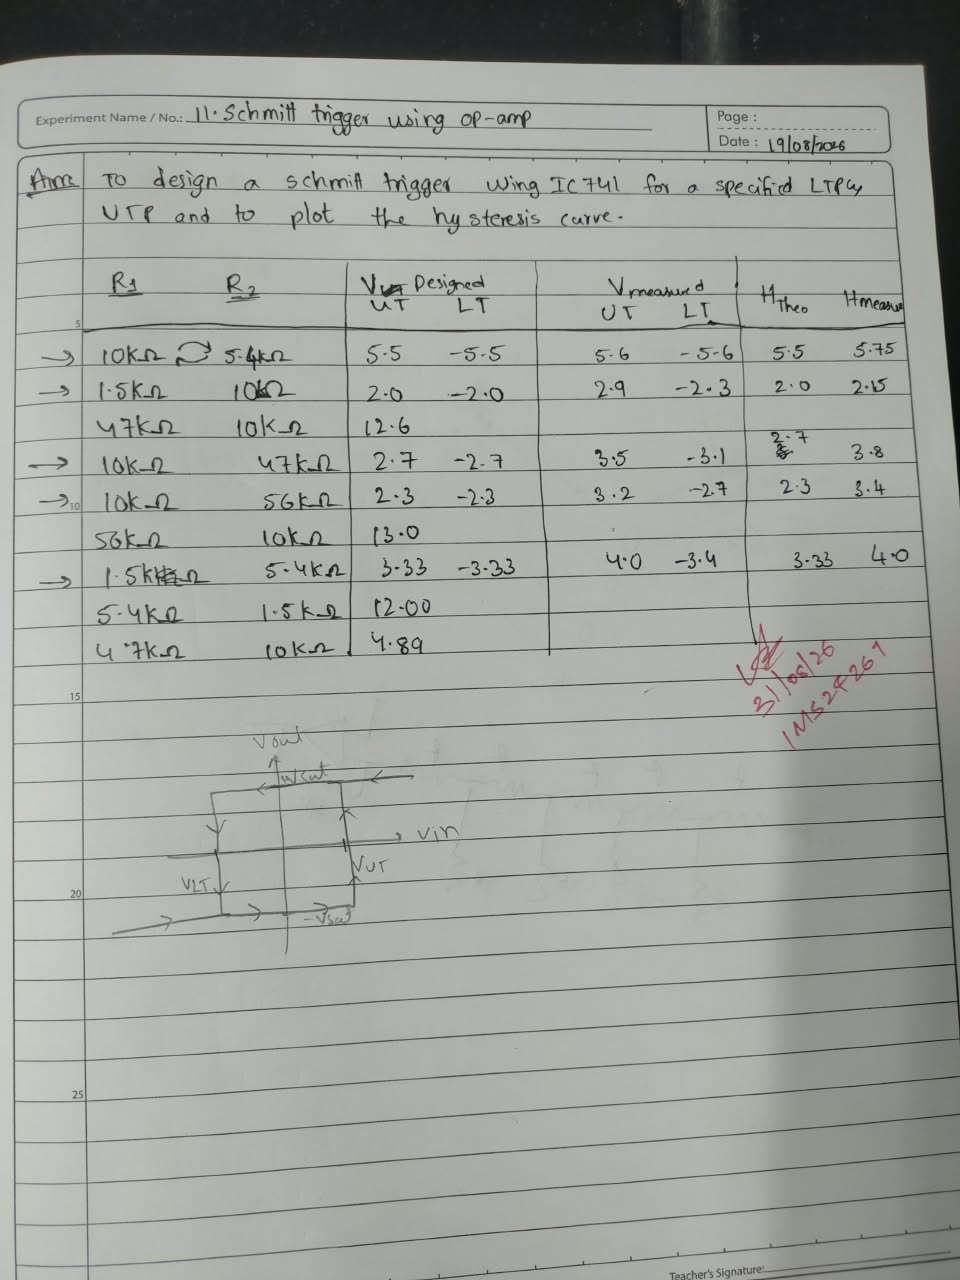
\includegraphics[width=0.85\textwidth]{../Lab-Observations/Lab readings.jpeg}
    \caption{Lab Notes for Schmitt Trigger Observations}
\end{figure}

\begin{figure}[H]
    \centering
    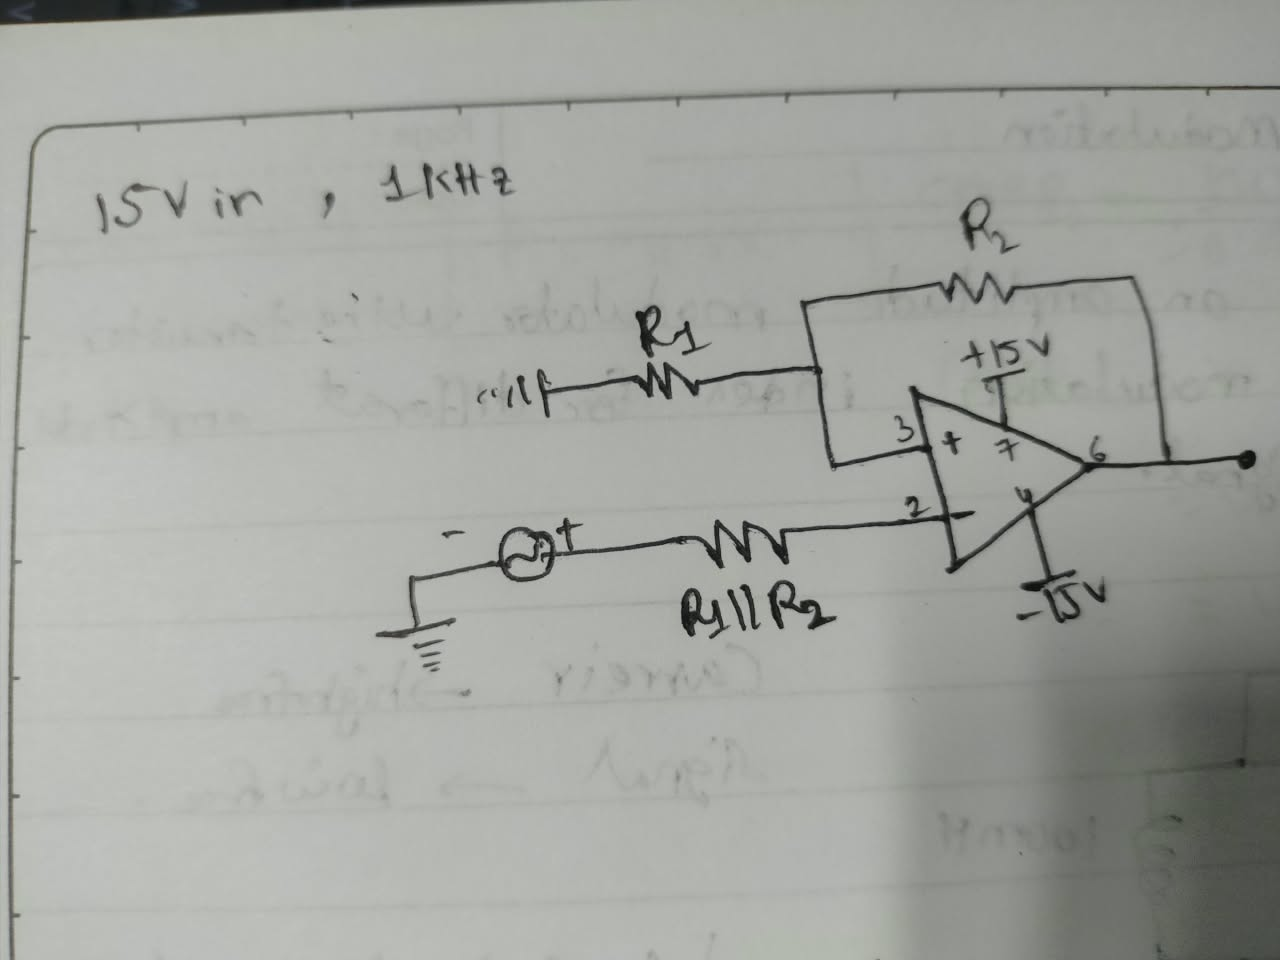
\includegraphics[width=0.85\textwidth]{../Lab-Observations/Circuit-digram.jpeg}
    \caption{Handwritten Circuit Diagram for Schmitt Trigger}
\end{figure}

\begin{figure}[H]
    \centering
    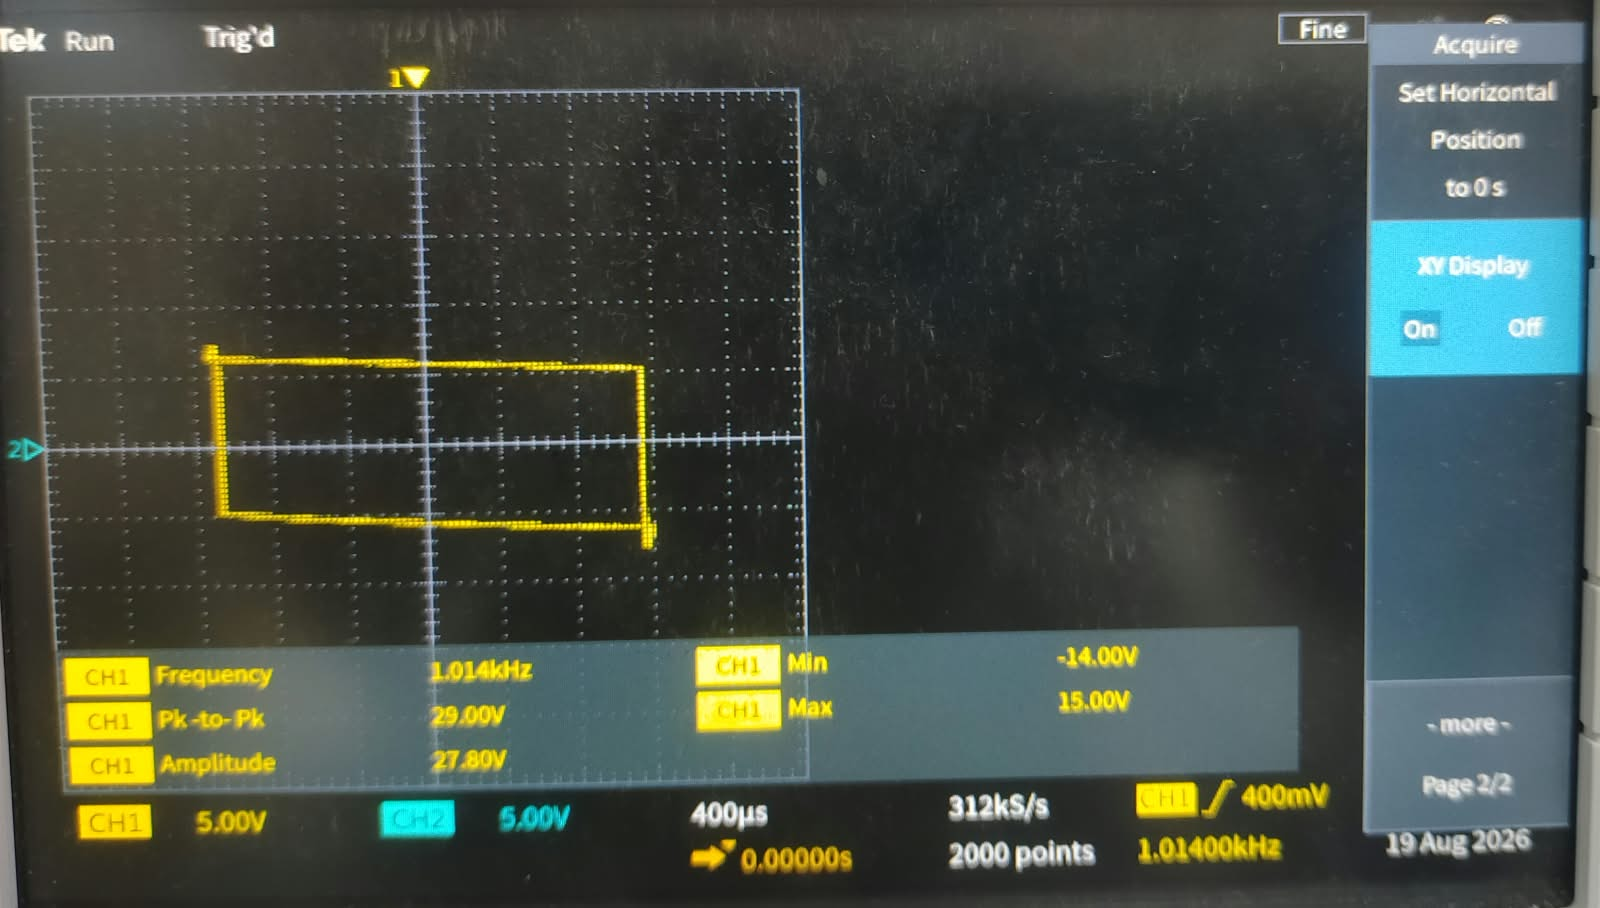
\includegraphics[width=0.85\textwidth]{../Lab-Observations/Observed hysterisis curve.jpeg}
    \caption{Oscilloscope trace showing the observed hysteresis curve in XY mode}
\end{figure}

\begin{figure}[H]
    \centering
    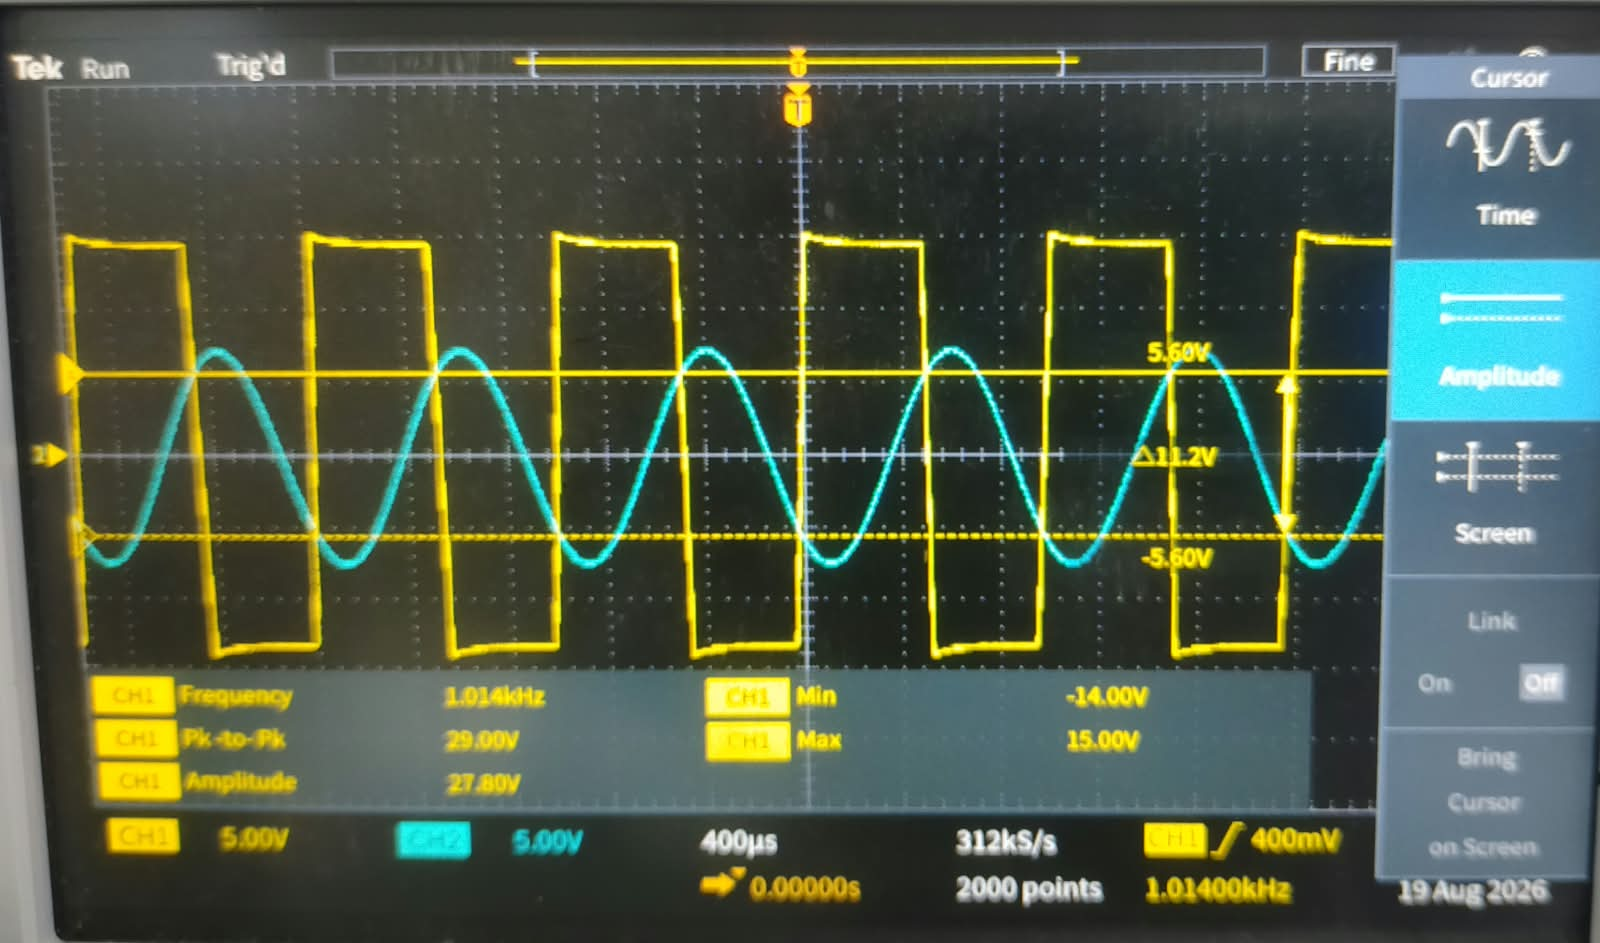
\includegraphics[width=0.85\textwidth]{../Lab-Observations/Schmitt-observed-wave.jpeg}
    \caption{Oscilloscope trace showing the input sine wave and the output square wave}
\end{figure}

\end{document}
